\subsection{Reports Module}
\par{The Reports module is used to provide statistical information that can be used by the lecture to observe overall usage of the forum and award rewards to users that participate constructively to the forum. Management can also use the data collected to make updates and maintain the system. The statistics module can be separated into the following layers:}

\subsection*{Personal Statistics}
\par{All users are able to view their own statistics and also stats related to the course modules they are participating in.}
\subsection*{User Statistics}
\par{Admin users will be able to view the statistics of individual users. These stats include the number of posts, likes, dislikes and overall participation.}
\subsection*{Course statistics}
\par{Admin users will be able to view statistics for a specified course module. These stats include the activity within a said period of time (ie: a week or month).}
\subsection*{Forum statistics}
\par{The statistics relating to overall forum activity is meant more for the platform administrators than the course module admin.}

\subsubsection{Use cases}
\par{The reporting module provides services to gather statistical information for each user and export a report back to the lecture, who can assess the user’s overall usage of the forum.}

\subsection*{getTotalPosts}
\par{The system will store the assessed user profile to generate a total for the number of posts a user has made. This statistical information will be saved and exported to the lecture/management.}
\subsection*{ComputeAverages}
\par{An effective way to present statistics is by representing them as averages over a given sample size. Factors like averagePostsPerWeek will be represented by averages across a collection of users for the said course module.}

\subsubsection{Domain Model}
\begin{figure}[h]
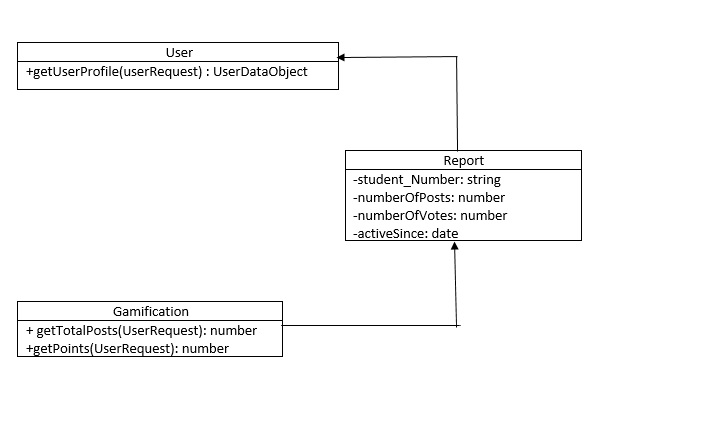
\includegraphics[width=\linewidth]
{Diagrams/report_domain_model.jpeg}
\caption {Domain model of the Buzz-Report module.}
\end{figure}
